\documentclass{beamer}
\usepackage[utf8]{inputenc}
\usepackage[export]{adjustbox}
\usepackage{hyperref}
\hypersetup{
	colorlinks=true,
	urlcolor=adcorange,
	linkcolor=adcblue
}

\usetheme{Madrid}

\title{Multiplayer trivia game}
\subtitle{HTML, CSS, JavaScript basics}
\author{Nathaniel Budijono}
\date{October 5, 2021}
\institute{UMN ADC}

\definecolor{adcblue}{RGB}{115,203,255}
\definecolor{adcorange}{RGB}{242,114,0}

\setbeamercolor{palette primary}{fg=white,bg=adcblue}
\setbeamercolor{palette secondary}{fg=adcorange,bg=white}
\setbeamercolor{structure}{fg=adcblue,bg=white}
\setbeamercolor{title in head/foot}{fg=adcblue,bg=white}
\setbeamercolor{date in head/foot}{fg=gray,bg=white}
\setbeamercolor{palette tertiary}{fg=white,bg=adcorange}

\begin{document}

\begin{frame}
    \titlepage
    \includegraphics[width=0.25\textwidth, right]{figs/ADC_Logo_Blue.png}
\end{frame}

\begin{frame}{Logistics...}
	Streaming
	\begin{itemize}
		\item \href{https://umn.zoom.us/my/adc.workshop}{https://umn.zoom.us/my/adc.workshop}
		\item Recordings will be posted as unlisted YouTube videos as linked at \href{https://adcumn.org/meetings}{https://adcumn.org/meetings}
	\end{itemize}

	\bigskip\pause

	In-person
	\begin{itemize}
		\item Tuesdays 5-6pm
		\item Tate Hall B20
	\end{itemize}
\end{frame}

\begin{frame}{Officer openings!}
	\begin{itemize}
		\item Workshop instructors
	\end{itemize}

	\bigskip

	DM us on the discord!

	\bigskip

	\href{https://z.umn.edu/ADCdiscord}{https://z.umn.edu/ADCdiscord}
\end{frame}

\begin{frame}{A look ahead...}
	\centering
	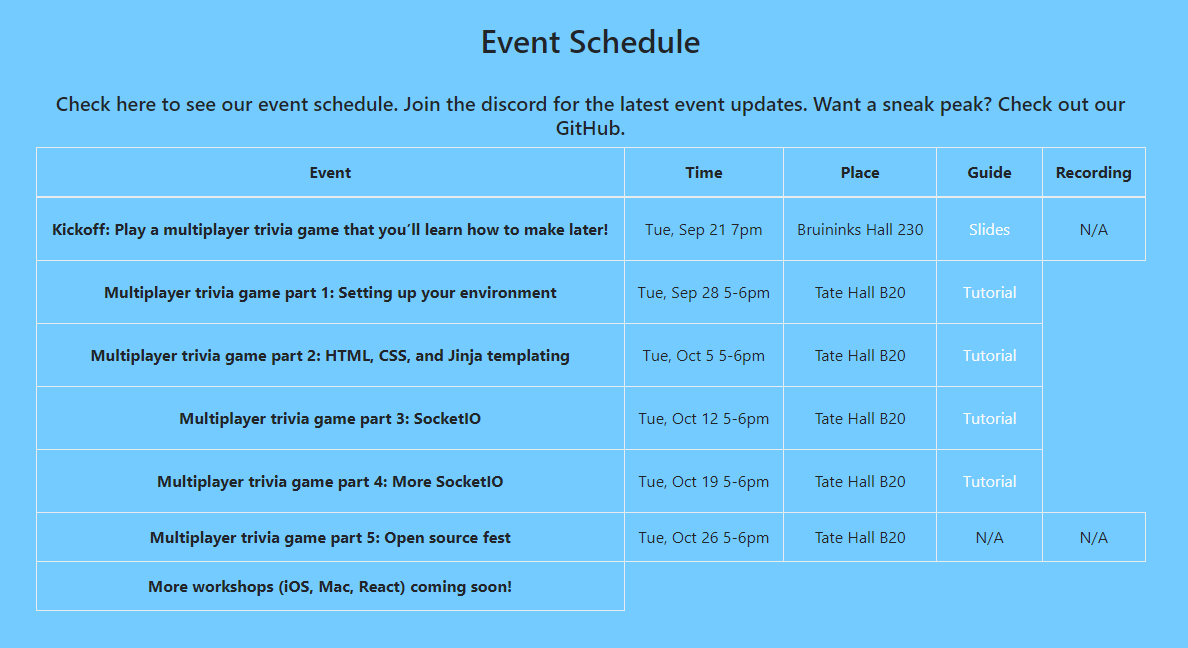
\includegraphics[width=0.9\textwidth]{figs/schedule.png}
\end{frame}

\begin{frame}{Follow the guide!}
	\centering
	\href{https://z.umn.edu/adc-mtg}{https://z.umn.edu/adc-mtg}

	\bigskip

	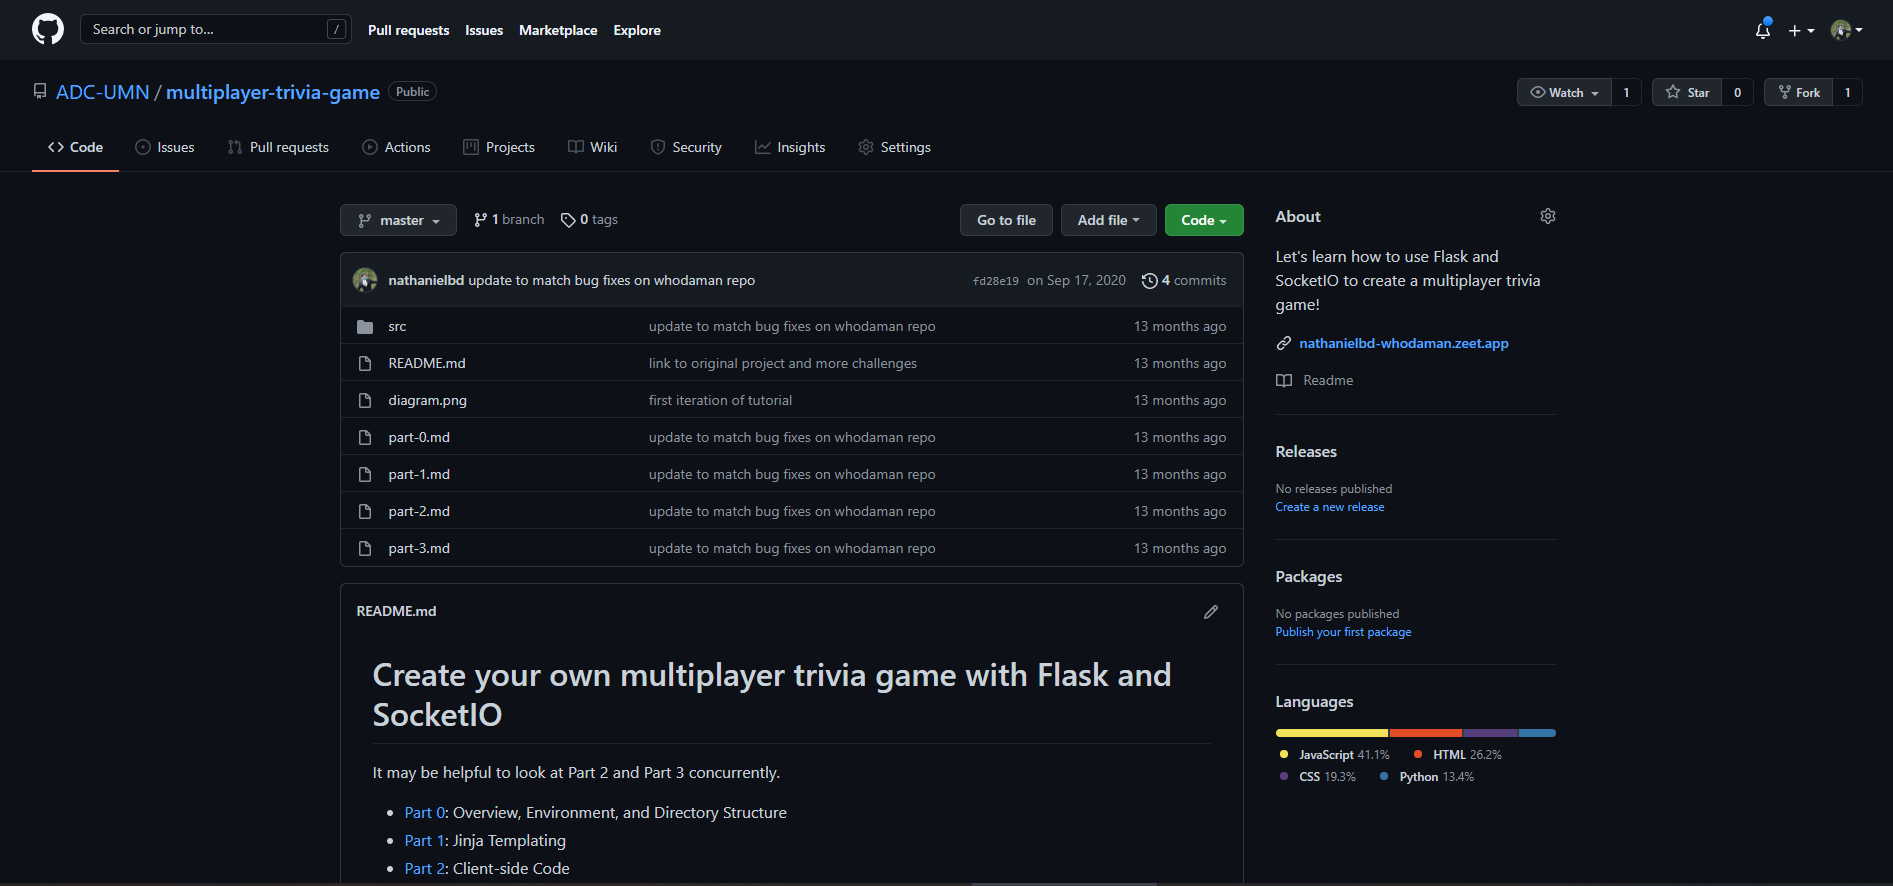
\includegraphics[width=0.9\textwidth]{figs/guide.png}
\end{frame}

\begin{frame}{Jinja Templating}
	\only<1>{
		\begin{columns}
			\begin{column}{0.5\textwidth}
				\centering
				\texttt{layout.html}
				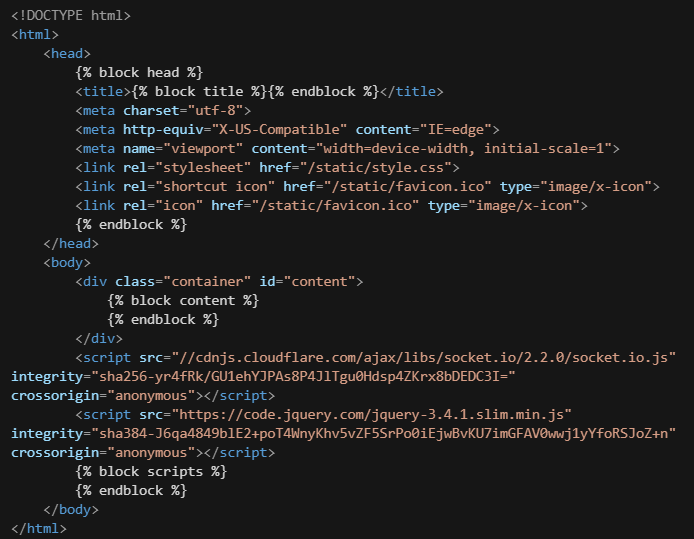
\includegraphics[width=0.9\textwidth]{figs/layouthtml.png}
			\end{column}
			\begin{column}{0.5\textwidth}
				\centering
				\texttt{admin.html}
				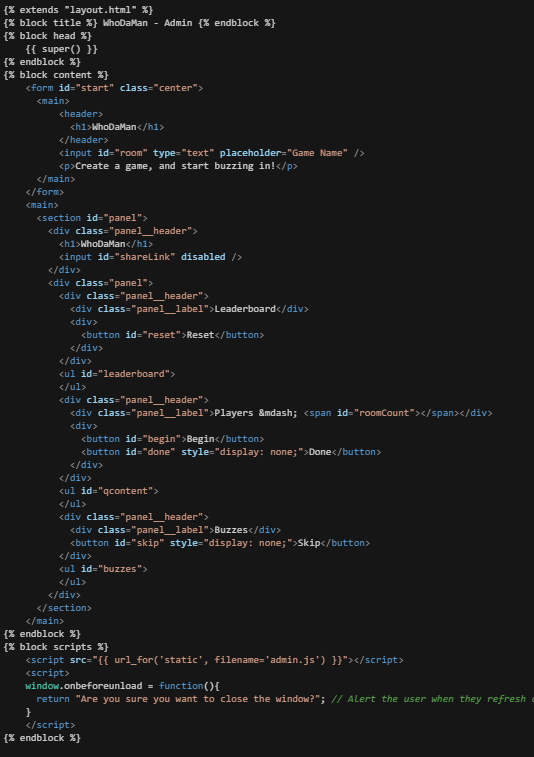
\includegraphics[width=0.9\textwidth]{figs/adminhtmlfull.png}
			\end{column}
		\end{columns}
	}

	\only<2>{
		\centering
		\texttt{app.py}
		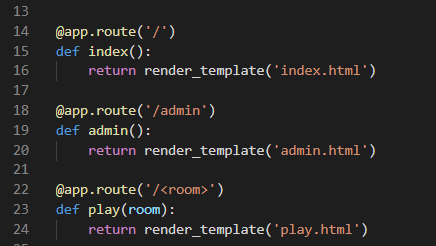
\includegraphics[width=0.9\textwidth]{figs/flask-routes.png}
	}
\end{frame}

\begin{frame}{Running the app yourself}
	Open the terminal!

	\bigskip

	Change to \texttt{/src}

	\pause

	\bigskip

	\begin{enumerate}
		\item \textbf{Create virtual environment}: \texttt{python3 -m venv env} \pause
		\item \textbf{Activate virtual environment}: \\ Linux/Mac: \texttt{source env/bin/activate}, \\ Windows: \texttt{env\textbackslash Scripts\textbackslash activate.bat} \pause
		\item \textbf{Install dependencies}: \texttt{pip install -r requirements.txt} \pause
		\item \textbf{Run app}: \texttt{python app.py}
	\end{enumerate}
\end{frame}

\begin{frame}{A question}
	In \texttt{admin.html}, how do we make \texttt{<form>} visible at the start, then hide it and show 
	\texttt{<main>}?

	\pause

	\bigskip

	CSS selectors and JQuery
\end{frame}

\begin{frame}{DOM manipulations}
	\only<1>{
		\centering
		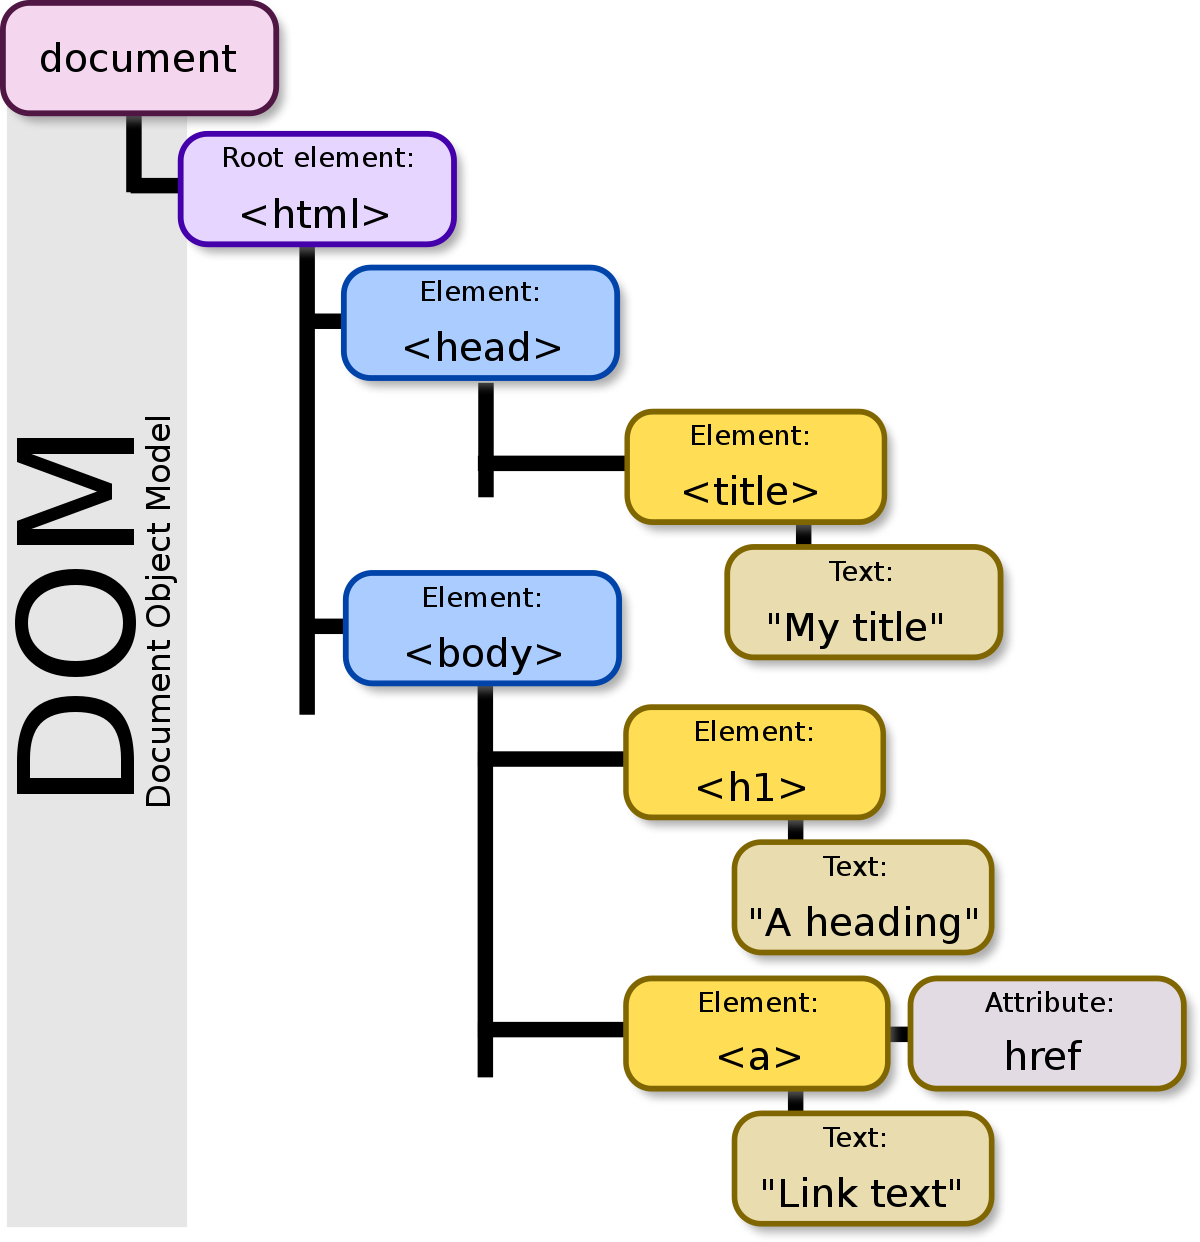
\includegraphics[width=0.6\textwidth]{figs/dom.png}
	}

	\only<2>{
		Notice the Jinja templating!
		\begin{columns}
			\begin{column}{0.5\textwidth}
				\centering
				\texttt{admin.html}
				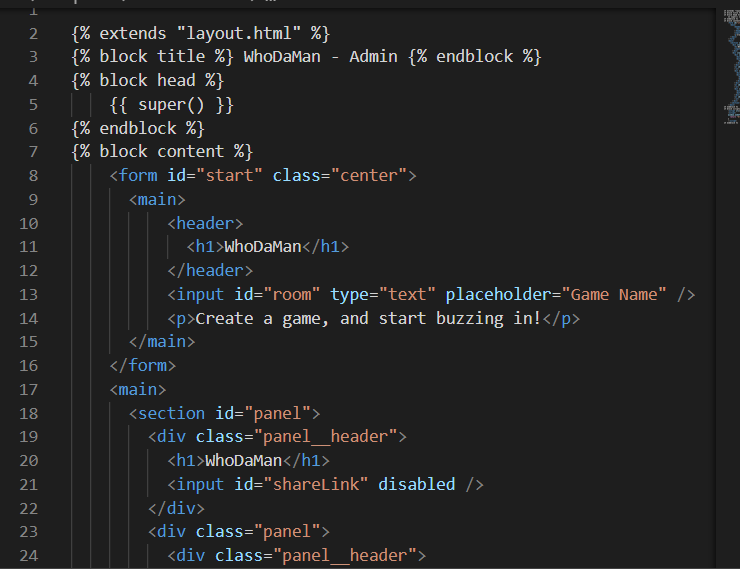
\includegraphics[width=0.9\textwidth]{figs/adminhtml.png}
			\end{column}
			\begin{column}{0.5\textwidth}
				\centering
				\texttt{admin.js}
				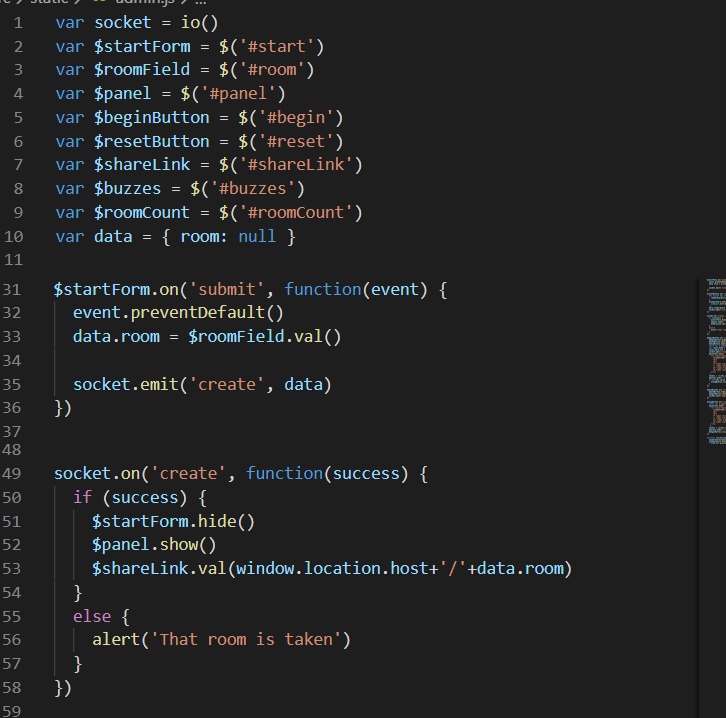
\includegraphics[width=0.9\textwidth]{figs/adminjs.png}
			\end{column}
		\end{columns}
	}
\end{frame}

\begin{frame}{CSS}
	\texttt{
		selector \{
			attribute: value;
		\}
	}

	\pause

	\bigskip

	\begin{center}
		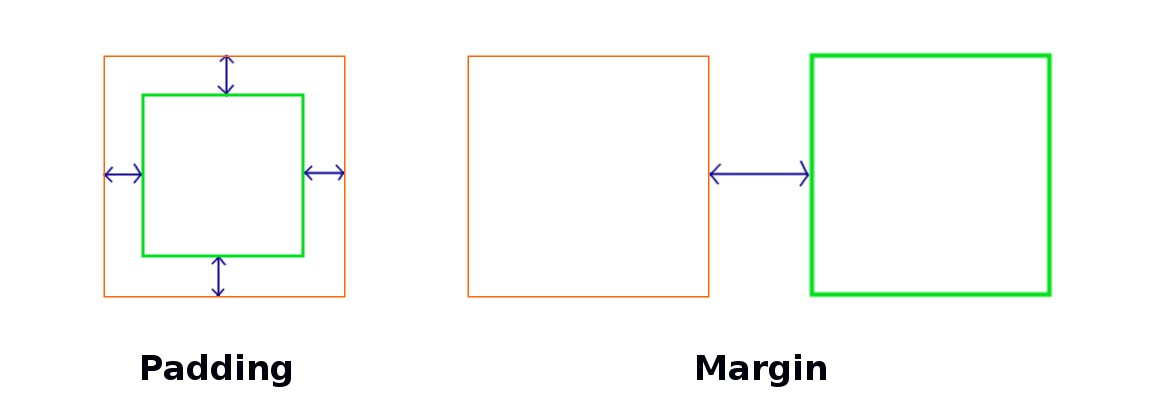
\includegraphics[width=0.9\textwidth]{figs/margin-padding.jpeg}	
	\end{center}

	\pause

	\bigskip

	Let's look at \href{https://github.com/ADC-UMN/multiplayer-trivia-game/blob/master/src/static/style.css}{\texttt{static/style.css}}!
\end{frame}

\begin{frame}{A challenge}
	Try fiddling around with the HTML and CSS.

	\pause

	\bigskip

	Some ideas:
	\begin{itemize}
		\item Create your own template that extends \texttt{layout.html} \pause
		\item Create a section in \texttt{admin.html} where live chat might go \pause
		\item Create a button that switches the page from light theme colors to dark theme colors
	\end{itemize}
\end{frame}

\end{document}